%%%%%%%%%%%%%%%%%%%%%%%%%%%%%%%%%%%%%%%%%%%%%%%%%%%%%%%%%%%%%%%%%%%%%%%%%%%%%%%%
%2345678901234567890123456789012345678901234567890123456789012345678901234567890
%        1         2         3         4         5         6         7         8

\documentclass[letterpaper, 10 pt, conference]{ieeeconf}  % Comment this line out if you need a4paper

%\documentclass[a4paper, 10pt, conference]{ieeeconf}      % Use this line for a4 paper

\IEEEoverridecommandlockouts                              % This command is only needed if 
                                                          % you want to use the \thanks command

\overrideIEEEmargins                                      % Needed to meet printer requirements.

%In case you encounter the following error:
%Error 1010 The PDF file may be corrupt (unable to open PDF file) OR
%Error 1000 An error occurred while parsing a contents stream. Unable to analyze the PDF file.
%This is a known problem with pdfLaTeX conversion filter. The file cannot be opened with acrobat reader
%Please use one of the alternatives below to circumvent this error by uncommenting one or the other
%\pdfobjcompresslevel=0
%\pdfminorversion=4

% See the \addtolength command later in the file to balance the column lengths
% on the last page of the document

% The following packages can be found on http:\\www.ctan.org
%\usepackage{graphics} % for pdf, bitmapped graphics files
%\usepackage{epsfig} % for postscript graphics files
%\usepackage{mathptmx} % assumes new font selection scheme installed
%\usepackage{times} % assumes new font selection scheme installed
%\usepackage{amsmath} % assumes amsmath package installed
%\usepackage{amssymb}  % assumes amsmath package installed



%\documentclass[conference]{IEEEtran}
% The preceding line is only needed to identify funding in the first footnote. If that is unneeded, please comment it out.

\usepackage{amsmath,amssymb,amsfonts}
\usepackage{algorithmic}
\usepackage{graphicx}
\usepackage{textcomp}
\usepackage{xcolor}
\usepackage{todonotes}
\usepackage{verbatim}
\usepackage{pgfplots}
\usepackage{comment}
\usepackage[super]{nth}
    
\setlength{\abovecaptionskip}{0pt plus 3pt minus 2pt}
\setlength{\abovedisplayskip}{2pt}
\setlength{\belowdisplayskip}{2pt}




\usepackage{tabularx}
\usepackage{color, colortbl}
\definecolor{Gray}{gray}{0.8}

\title{\LARGE \bf
What Information Should a Robot Convey
}
%DS - I shortened the title to be on one line to save some space. If you had your heart set on the other title you can change it back.

%\author{Hooman Hedayati$^{1}$ and Daniel Szafir$^{2}$% <-this % stops a space
%\thanks{$^{1}$Department of Computer Science, University of Colorado Boulder.
%        {\tt\small hooman.hedayati@colorado.edu}}%
%	\thanks{$^{2}$Department of Computer Science and ATLAS Institute, University of Colorado Boulder.
%		{\tt\small daniel.szafir@colorado.edu}}%
%}

\author{Blank for Review}


\newcommand\dan[1]{\textcolor{red}{DS--#1}}
\newcommand\hooman[1]{\textcolor{red}{HoOman--#1}}


\begin{document}


\maketitle

\thispagestyle{empty}
\pagestyle{empty}


%%%%%%%%%%%%%%%%%%%%%%%%%%%%%%%%%%%%%%%%%%%%%%%%%%%%%%%%%%%%%%%%%%%%%%%%%%%%%%%%
\begin{abstract}
%\hooman{I think the main contribution of the paper is a list of items users want to know about the robot. this list helps designers to have users need in mind. the reason why this list is important is that people get uncomfortable soon if they can not understand a situation e.g. if I'm with a group of people that I don't know their language I get uncomfortable easily. this is the main point if wanted to say in abstract}
Robotic technologies are becoming increasingly pervasive within industrial and domestic settings, resulting in more frequent interactions between humans and robots. In order to ensure these interactions are effective, the field of Human-Robot Interaction (HRI) has argued that robots and humans must establish a shared common ground by communicating fundamental pieces of information to each other, such as their intentions, goals, plans, status, etc. While a relatively large body of work has explored how robots might signal individual aspects of such information to users, we still know relatively little regarding the relative importance of such information overall (e.g., is communicating robot status more important than robot goals?). Such information is necessary for robots acting in the wild to enable creating prioritized lists of communicative goals as, at any given time, it is unlikely that a robot will be able to convey all possibly relevant or important aspects of information to users. Prioritizing information for users is a complex problem as many factors might influence information priority, including task context, user expertise, and robot capability. In this work, we take an initial step towards understanding prioritization by exploring what types of information users request, and how the rankings of informational importance that users assign change, in a prototypical shared-environment interaction with three different types of robots. Our results, collected from 150 participants on Amazon's Mechanical Turk, generally found that users value information related to the robot's battery, capabilities, task, safety, navigation, communication, and privacy, with user priorities of these items varying across a small ground robot, a large ground robot, and an aerial robot.  %We made videos of a user interacting with 3 different robots, a small size ground robot, a big size ground robot with manipulator and an aerial robot and created a "priority list" consist of possible information a user might want to know and designed a survey in which participants must rank the information they want to know. We recruited 150 participants on Mechanical Turk and share our finding as a list of the user's priorities in the result section. Provided list might help robot designers to design robots with users' need in mind.
\end{abstract}


%%%%%%%%%%%%%%%%%%%%%%%%%%%%%%%%%%%%%%%%%%%%%%%%%%%%%%%%%%%%%%%%%%%%%%%%%%%%%%%%
\section{INTRODUCTION}
People are increasingly integrating robots into work practices for a wide variety of domestic, commercial, and government uses. For example, aerial robots may be used for structural inspection \cite{chan2015towards} and package delivery \cite{d2014guest}, while mobile industrial robots can navigate factory and warehouse floors to move payload \cite{wurman2008coordinating} or perform various manipulation tasks \cite{datta2008development, hvilshoj2011little}. In addition, social service robots are emerging as a means of providing human assistance in customer service related tasks (e.g., welcoming, guiding, taking orders, delivering, etc.) in shopping centers, restaurants, and hotels \cite{acosta2006design, datta2011pilot, kanda2009affective, osawa2017real, zalama2014sacarino}. In the household, robots may help with cleaning \cite{forlizzi2006service}.

One commonality in many of these emerging use cases for robotics is that they require robots to operate in shared spaces with human users. As a result, such robot deployments will increasingly depend on designing robots that are able to successfully navigate the intricacies of human-robot interactions, ranging from coexistence, to coordination, to collaboration \cite{cha2018survey}. 

Achieving the ultimate goal of designing robots that provide smooth, safe, enjoyable, intuitive, and productive interactions with users will require that robots communicate with humans to some degree \cite{cha2018survey, khatib1999robots}. %In a human-human interaction, people are good at interpreting the signals coming from the opponent e.g., if two people passing by each other in a narrow hallway, often they are good at signaling/interpreting signal which path ( right or left ) are they going to take. If they can not perform a good job, the mentioned interaction would become an awkward situation. For a good interaction, both human and robot should have a basic understanding of each other. It is essential for a human to know more about the state of the robot and it is necessary for the robot to convey needed information to the user.
Prior work in the human factors and human-robot interaction (HRI) communities have explored various aspects of human mental model formation \cite{aggarwal2011human}, specific aspects of information communication \cite{arras2005we, bauer2008human}, and what signals to use to convey specific information \cite{cha2018survey}. As an example, prior work has explored several methods to convey robot motion intent (i.e., ``where will the robot move next''), including the use of expressive motion \cite{Zhou:2017}, electronic signaling lights \cite{szafir2015communicating}, sound \cite{cha2018effects}, and augmented reality cues \cite{walker2018communicating,hedayati2018improving,8673306}. 

While this past work helps us understand the question of ``what medium might a robot use to signal specific information?'' it does not necessarily help us understand the broader question of ``what information should a robot convey to users?'' In this paper, we focus on this second question as, other than for specific use cases such as designing a bomb defusing robot \cite{adams2005human}, to the best of our knowledge, how robots might prioritize what information to communicate to users has yet to be deeply explored by robot researchers or designers.

As a first step towards exploring this question, we recruited 150 participants using Amazon's Mechanical Turk that were evenly divided into three groups. Each group of 50 participants watched a short video depicting a user interacting with one of three different robots (small ground robot, large ground robot, or aerial robot) in a shared environment. Users were then asked what information they would have liked the robot to convey and how important they felt each aspect of information might be were they to interact with the robot they saw in the future. Our overall methodology of online data collection follows that of several promising HRI studies in recent years \cite{Song:2018,hoffman2019,Zhou:2017}, and, while there are limitations to data that is collected online, we believe our results may may provide initial insights for robot designers and help inform future work that further explores the space of understanding how robots can prioritize information for users. %provide initial insight into user preferences regarding information prioritization. 
Below, we describe the data collection methodology and analysis of our results in more detail.

\section{Survey and Procedure} \label{survey}

\begin{figure*}
\centering
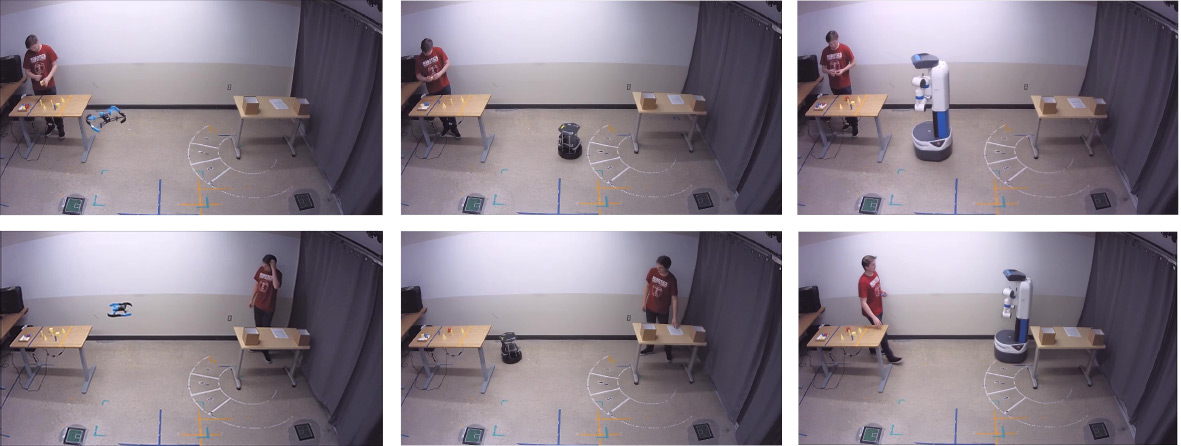
\includegraphics[width=\textwidth]{figures/task3robots.jpg}
\caption{Screenshots of videos shown to users as part of the survey in which a user interacts with a robot in a shared environment. Top: robots do not block the path of the user. Bottom: robots require the user to navigate around them. Left: aerial robot, Middle: small ground robot, Right: large ground robot.}
\label{fig:task}
\end{figure*}

We designed a survey with 4 sections to gain insights into what sorts of information users might find most valuable for a robot operating in a shared environment to communicate. In the first section, participants watched two short videos, each approximately 30 seconds in duration. Both videos depicted a user completing a pick-and-place task while sharing an environment with one of 3 robots (Figure \ref{fig:task}). There are two tables in the environment. One table contains the user instructions and two boxes, while the other table contains various wooden blocks with associated numbers. The instructions required the user to follow a sequence of steps in which they selected a specified block from one table and placed it in one of the boxes in the other table (e.g., ``1. The yellow pyramid with number 15 should go in Box A"). 
    
In both videos, the robot acted as a supervisor, which meant that it occasionally navigated close to the tables to inspect the current status of the task (e.g., how many objects were in a box or whether objects were placed in the correct box). In the first video, the robot was on the opposite side of the table and completely isolated from the user (Figure \ref{fig:task} top images). However, in the second video, the robot went the same side of the table as the user and thus at times required the user to navigate around the robot (Figure \ref{fig:task} bottom images). Our goal in designing these two videos was to highlight scenarios in which users may coexist in shared environments with robots (i.e., bystander interactions) as well as scenarios requiring more direct interaction (e.g., to resolve right-of-way issues) as the information that users desire from the robot may depend on the amount and type of interaction. %We designed the videos to mimic two scenarios, in the first one the user and aerial robot are just in the same space there is not any interaction between them, but at the same time there couple of question that the user might want to know about the robot. In the second video, there is actually an interaction between them, the robot is on the way of the user and in this case.

After watching the videos (which participants could re-watch any amount of times at any time during the survey), participants produced a rank order for a number of items that each corresponded to some aspect of information that a robot might convey, placing the items in order of how important the participant perceived this information to be were they to interact with the robot as in the videos they had just watched. Users were required to rank 22 items for the aerial robot and 21 items for the ground robots; all items were identical across all three robots, except for the addition of an item corresponding to ``The robot conveying when it will change its altitude" that was only included for the aerial robot (as it was not applicable to the ground robots). These items, provided in Table \ref{table:itemslist}, were created by reviewing prior HRI literature examining what types of information robots might signal to users and a series of brainstorming sessions with expert roboticists with at least 5 years of experience.

\begin {table}
\begin{center}
\caption{Survey Rank Items}
\label{table:itemslist}
\vspace{1em}
\begin{tabular}{|p{8pt} | p{215.6pt} |}
 %\hline
 %\multicolumn{2}{|c|}{List of all items} \\
 \hline
 \# & The robot conveying ... \\
 \hline
1 & whether it is currently acting autonomously or being controlled by a person.\\
\hline
2 &  whether or not it is safe to get close to it.\\
\hline
3 &  what it knows about the surrounding environment (i.e., the objects and people it can sense).\\
\hline
4 &  whether or not it needs assistance.\\
\hline
5 &  whether or not any faults/errors are detected (e.g., electric circuits damaged, etc).\\
\hline
6 &  whether or not its camera is recording.\\
\hline
7 &  when and in what direction robot would move next.\\
\hline
8 &  its battery life remaining in time (hours/minutes/seconds).\\
\hline
9 &  whether or not there is a problem with the engines/motors.\\
\hline
10 &  whether or not it currently knows where you are.\\
\hline
11 &  its current task progress (as a percentage of the whole task).\\
\hline
12 &  its wireless signal strength.\\
\hline
13 &  contact information for how to leave feedback about the robot.\\
\hline
14 &  a list/schedule of upcoming/planned tasks (task queue).\\
\hline
15 &  the name of its current task along with a short description.\\
\hline
16 &  a list of successfully/unsuccessfully completed tasks (task history).\\
\hline
17 &  its remaining battery life as a percentage.\\
\hline
18 &  its most recent maintenance report (e.g., last time propeller was changed).\\
\hline
19 &  the current time and date.\\
\hline
20 &  how to look up more information about the robot (e.g., where to find a manual).\\
\hline
21$^{\circ}$ & its total mission duration (from start to the current moment).\\
\hline
21* &  its total flight duration (from takeoff to the current moment).\\
\hline
22* &  when it will change its altitude.\\
\hline

\end{tabular}
\begin{tabular}{|p{236pt}|}
 $\circ$ Only showed for small and large ground robot surveys\\
 * Only showed for aerial robot survey\\
\hline
\end{tabular}

\end{center}
\end{table}
    
The list of items was created to be as comprehensive as possible without including redundant items. At a high level, the items on the list can be categorized into five groups. As Cha et al. \cite{cha2018survey} suggests, \textit{condition} and \textit{activity} form the first two groups. \textit{Condition} refers to items corresponding to information the robot might convey about itself, such as ``The robot conveying when and in what direction robot would move next'' etc. The second group \textit{activity} represents information that the robot might convey about the task it is doing, for example ``The robot conveying a list of successfully/unsuccessfully completed tasks (task history)'' or ``The robot conveying whether or not any faults/errors are detected (e.g., electric circuits damaged, payloads/sensors not mounted correctly, etc.).'' In addition to these two groups, we developed three new categories: 
\begin{itemize}
    \item \textit{Safety} corresponds with information related to whether it is safe and/or appropriate for humans to interact closely with the robot, such as ``The robot conveying whether or not it is safe to get close to it'' or ``The robot conveying whether or not it currently knows where you are.''
    
    \item \textit{Privacy} represents information about the data the robot may be collecting about the user; an example for this group is ``The robot conveying whether or not its camera is recording.''
    
    \item \textit{Communication} focuses on information the robot might communicate that is related to the context of the task, for example ``The robot conveying whether or not it needs assistance.''
    
\end{itemize}  

For each participant, the list of items was presented to participants in randomized order to reduce the potential for initial placement (i.e., rank) bias. Participants were tasked with re-ordering the list of items in order of their perceived priority.  
    
In the next section, participants were asked to provide a 1--7 Likert-type rating regarding their perceived importance for each item they ranked in the previous section. Here 1 was defined as ``not important'' and 7 was defined as ``very important.'' This section of the survey served two primary purposes. First, this section helped provide supplementary information on perceptions of absolute importance to contextualize the information on relative importance from the previous section (e.g., even items ordered near the end might be perceived as highly important by participants). Second, these questions provided a validation method for the items in the previous section (i.e., items ranked lower in the prior section should receive an equal or lower score in this section compared to items that were ranked as relatively more important). This validation helped us identify and control for the quality of participant responses. %Although it might seem like an unnecessary and redundant question, it is really important as a validation method. Using ranking question with more than 5 items is not suggested as people might not remember all the items in the list. In these cases the first and the last couple of items in the ranking are reliable, but the data in the middle might be noisy as a result not remembering the whole list. Since our list for ranking has more than 5 items, we used the second question for validation. The answers to the ranking question should have the same trend as the second question does. As an example, if the first item on the ranking should have higher or at least the equal as compare to the last item in the ranking answer. This help to remove the answers which are not consistent.

While we created a large sample of items corresponding to different types of information it may be useful for a robot to convey, we recognize that our list may not be exhaustive and might be missing potentially critical elements. As a result, the next section of the survey provided participants with open-ended questions where participants could suggest any other information they think would be helpful to know about the robot or useful for the robot communicate to them. For each suggestion, we also asked participants to provide a Likert-type rating of 1--7 regarding how important they believe this suggested information might be. Each participant had the option to provide and rate 3 new suggestions. %The question asked to give us a better understanding of what a user wants and how important is that feature for that user. 

In the last section of the survey, we collected demographic information regarding participant age, gender, education and the level of prior familiarity with robots. We also included a question about obvious features in the two videos for additional quality control (this question asked for the number of boxes on the table in order to ensure that participants actually watched the videos).

With IRB approval, we deployed the survey on Amazon Mechanical Turk and collected responses from 186 participants. After initial validation analysis, we removed data from 36 participants who didn't pass the video sanity check or demonstrated inconsistencies across the ranking and rating sections. %Which mean their first item in ranking question has a lower likert score in the second question than their last item in the ranking. e.g., one participant's first rank is "The robot conveying whether or not there is a problem with the engines/motors." with 4 as a score, and the last item in the ranking is  "The robot conveying the current time and date." with 6 as a score. 
As a result, we ended up with 150 responses for full analysis.

\section{Results}
In this section, we describe the population demographics and level of familiarity with the robot for each of the 3 groups. We then provide a table with the average of participants' top five and bottom five choices in their relative rankings of priority. We focus on the top and bottom five items due to high noise amongst middling ranked items. These lists were created by averaging participant scores for every item across all responses (i.e., 1 would refer to the item ranked most important and 22 would be the item ranked least important).

After sorting the data, we found that the difference between the mean rankings of any two consecutive items was quite small on average $(\Delta_{i,i+1} \leq 0.5)$. However, we observed certain larger gaps between items $(\Delta_{i,i+1} > 0.5)$, which we highlight in the respective tables. %As an example in the ``Most important" table (top table) in \ref{table:bebop} there is a gap between the \nth{3} item and \nth{4} one, since $\Delta_{i_3,i_4} = 0.8 $. The \nth{1}, \nth{2} and \nth{3} items are colored in light gray to emphasize they are the most important items for the participants, the same idea for the ``Least important" table (bottom table) in \ref{table:bebop} shows that the items \nth{20}, \nth{21} and \nth{22} are the least important in the participants point of view.

As mentioned in Section \ref{survey}, all the ranked items belong to one of the following categories: Safety, Activity, Communication, Privacy, or Condition. For each robot we also report on the average rank of each category to provide insight regarding the perceived relative importance of these categories of information overall. 

Finally, we explore the participants' responses to the open-ended questions and their suggestions for additional information that the robot might convey. For the open-ended questions, all participant responses were given to two annotators who were separately tasked with categorizing the answers. The annotators freely chose the number of categories and created a name for each category. The annotators independently identified the same number of categories which also matched in terms of general themes, although the specific name of each category was not identical (e.g., the first annotator termed one set of responses ``interaction,'' while the second annotator grouped the same responses but named the category ``communication''). After this process we met with each annotator to confirm the intended theme of each category and determine a final category name, resulting in: \textit{Navigation}, \textit{Battery}, \textit{Safety}, \textit{Task}, \textit{Robot Capabilities}, \textit{Interaction} and \textit{Privacy}. Based on the annotators' explanations, we determined that \textit{Navigation} and \textit{Battery} represented new groups, while the \textit{Task} category is analogous to the \textit{Activity} category from our initial group of the items we provided to participants to rank. Similarly, \textit{Robot Capabilities} matched \textit{Condition} and \textit{Interaction} matched \textit{Communication}. 

The annotators exhibited good level of agreement regarding on the items identified for each category, the Cohen's $\kappa$ = 0.639 which shows the strength of agreement is considered to be good. However, there were a few responses that the annotators didn't agree on, such as \textbf{Participant 42 (large ground robot):} ``Speaking out loud what it's current task is.'' For this suggestion, the first annotator put it under \textit{Task} category while the second annotator categorized it as \textit{Interaction}. We think the both categories are valid, since the participant's response is ambiguous by the nature and it may be interpreted both as information about the task and also about the interaction. %\hooman{talk about that we didn't expect much from the open ended question since the priority list was complete in our point of view} The result are as follows:

\subsection{Small ground robot}
Among valid responses, 12 participants identified themselves as female while 38 identified as male. Average participant age was 31.4 (SD = 7.1), with a range of 20--59. On a seven-point scale, participants reported a moderate prior familiarity with robots (M = 3.8, SD = 1.5). The ranking results are presented in Table \ref{table:turtlebot}. Safety was the most important category for participants while Condition was the least important. Among categories, Safety (M = 5.5) was ranked most important on average, followed by Privacy (M = 9.5), Activity (M=10.8), Communication (M = 12.5) and Condition (M = 16.6).
    
\begin {table}[h]
\begin{center}
\caption{List of the most/least important items based on participant rankings for a small ground robot}
\label{table:turtlebot}
\vspace*{0.2 cm}
\begin{tabular}{|c|p{150pt}|c|c|}
 \hline
 \multicolumn{4}{|c|}{Most important} \\
 \hline
  Rank & The robot conveying ... & Mean & SD \\
 \hline
 \rowcolor{Gray}
1 & whether or not it is safe to get close to it. & 5.5 & 5.2\\
\hline
2 & when and in what direction robot would move next. & 8.3 & 6.0\\
\hline
3 & its current task progress (as a percentage of the whole task). & 8.3 & 4.5\\
\hline
4 & whether or not it needs assistance. & 8.8 & 5.7\\
\hline
5 & whether it is currently acting autonomously or being controlled by a person. & 8.9 & 5.8\\
\hline
\end{tabular}

\vspace*{0.5 cm}

\begin{tabular}{|c|p{150pt}|c|c|}
 \hline
  \multicolumn{4}{|c|}{Least important} \\
 \hline
  Rank & The robot conveying ... & Mean & SD \\
 \hline
   % \rowcolor{Gray}
17 & The robot conveying its wireless signal strength. & 14.2 & 4.7\\
\hline
   %\rowcolor{Gray}
18 & how to look up more information about the robot. & 14.3 & 5.7\\
\hline
   %\rowcolor{Gray}
19 & the current time and date. & 14.9 & 5.6\\
\hline
   %\rowcolor{Gray}
20 & its remaining battery life as a percentage. & 15.4 & 5.1\\
\hline
   %\rowcolor{Gray}
21 & contact information for how to leave feedback about the robot. & 15.7 & 4.9\\
\hline
\end{tabular}
\end{center}
\end{table}

For the open-ended questions, 38 suggestions were provided from 27 participants (M = 1.4 per participant). 19 participants provided one suggestion, 5 provided two suggestions, and 3 participants provided 3 suggestions. Both annotators found 2 of the responses invalid. The responses were random sentences with a robot keyword from a famous robotic book. Annotators grouped the responses in the following categories: battery (11.0\% of total responses, mean importance = 4.5) , robot capabilities (16.6\%, importance = 5.2), task (16.6\%, importance = 4.0), safety (8.3\%, importance = 7.0), navigation (19.4\%, importance = 5.4) and interaction (27.7\%, importance = 5.7). Examples of user responses that are representative of each category are presented below:


\begin{enumerate}
\item Battery
    \begin{itemize}
        %\item  \textbf{P25 (importance = 5):} ``How much time is on the battery under  workload."
        \item  \textbf{P47 (importance = 4):} ``Its estimated battery life and if it can complete the current project on said battery."
        \item  \textbf{P50 (importance = 5):} ``Robots battery level is enough to complete listed tasks"
    \end{itemize}
    
\item Condition
    \begin{itemize}
        \item  \textbf{P30 (importance = 5):} ``How much weight it can carry"
        \item  \textbf{P18 (importance = 4):} ``What features it has/what it is able to do"
        %\item  \textbf{P44 (importance = 5:} ``instructions about allowed interactions with the person."
    \end{itemize}

\item Activity
    \begin{itemize}
        \item  \textbf{P54 (importance = 6):} ``If there is a problem with the current task."
        %\item  \textbf{P38( importance 6:} ``I would like to know if there are any possible issues as to whether or not the robot won't be accomplishing the current task it's doing.  For example, if it's picking up an object - I'd want to know if there's possibly an issue with it such as the object is too heavy or something."
        \item  \textbf{P17 (importance = 4):} ``How many tasks are to be completed for the week."
    \end{itemize}
    
\item Safety
    \begin{itemize}
        %\item  \textbf{P21 (importance = 3):} ``An indication (audio or visual) if you are in the robots intended path. A beep or something like that would probably be very annoying after a short time, but a flashing light on a pole would probably work just fine."
        \item  \textbf{P7 (importance = 7):} ``How to shut it down if there was an emergency."
        \item  \textbf{P9 (importance = 7):} ``I'd like information on how to quickly shut it down in an emergency"
    \end{itemize}
    
\item Navigation
    \begin{itemize}
        \item  \textbf{P46 (importance = 7):} ``When the robot will move again."
        \item  \textbf{P23 (importance = 6):} ``To know where the robot's intended destination happens to be"
        %\item  \textbf{P21 (importance = 7:} ``Some indication (1 second ahead of time or so) of when the robot is about to move so that it's movements are telegraphed and you can expect movement."

    \end{itemize}

\item Communication
    \begin{itemize}
        \item  \textbf{P38 (importance = 7):} ``If it knows how to do whatever I'm requesting."
        \item  \textbf{P53 (importance = 5):} ``If it is waiting for me to do something"
        %\item  \textbf{P28 (importance = 3):} ``whether it needs any other kind of assistance"
    \end{itemize}
    
\end{enumerate}

\subsection{Large ground robot}
Among valid responses, 14 participants identified themselves as female while 36 identified as male. Average participant age was 31.8 (SD = 6.9), with a range of 22--59. On a seven-point scale, participants reported a moderate prior familiarity with robots (M = 4.2, SD = 1.4). The ranking results can be found  in Table \ref{table:fetch}. Similar to the results for the small ground robot, for the large ground robot we found that safety was the most important perceived concern of the participants, with robot capabilities ranked as the least important information for the robot to convey. Likewise, across categories information related to Safety (M = 5.8) was ranked as the most important, followed by Privacy (M = 7.0), Activity (M = 11.0), Communication (M = 12.0) and Condition (M = 17.1).

\begin {table}[h]
\begin{center}
\caption{List of the most/least important items based on participants ranking for Large ground robot}
\vspace{1em}
\label{table:fetch}
\begin{tabular}{|c|p{150pt}|c|c|}
 \hline
 \multicolumn{4}{|c|}{Most important} \\
 \hline
  Rank & The robot conveying ... & Mean & SD \\
 \hline
   \rowcolor{Gray}
1 & whether or not it is safe to get close to it. & 7.2 & 6.1\\
 \hline
2 & when and in what direction robot would move next. & 8.1 & 5.5\\
 \hline
3 & whether or not it needs assistance. & 8.3 & 5.6\\
 \hline
4 & whether or not it currently knows where you are. & 8.3 & 5.4\\
 \hline
5 & whether or not its camera is recording. & 9.1 & 4.1\\
 \hline
\end{tabular}

\vspace*{0.5 cm}

\begin{tabular}{|c|p{150pt}|c|c|}
 \hline
  \multicolumn{4}{|c|}{Least important} \\
 \hline
  Rank & The robot conveying ... & Mean & SD \\
 \hline
 
 % \rowcolor{Gray}
17 & how to look up more information about the robot. & 13.8 & 4.9\\
\hline
%   \rowcolor{Gray}
18 & The robot conveying its remaining battery life as a percentage. & 14.0 & 5.8\\
\hline
%   \rowcolor{Gray}
19 & The robot conveying its most recent maintenance report. & 14.0 & 5.3\\
\hline
%   \rowcolor{Gray}
20 & The robot conveying the current time and date. & 14.8 & 5.3\\
\hline
%   \rowcolor{Gray}
21 & The robot conveying contact information for how to leave feedback about the robot. & 16.4 & 4.8\\
\hline
\end{tabular}
\end{center}
\end{table}

We received 40 responses to the open-ended questions from 26 participants (M = 1.5 per participant). 14 participants provided a suggestion, 5 provided two suggestions, and 4 participants provided 3 suggestions. Annotators grouped the responses in the following categories: battery (5.0\% of total responses and mean importance = 4.5), robot capabilities (5.0\%, importance = 5.0), task (22.5\%, importance = 5.2), safety (15.0\%, importance = 6.1), navigation (15.0\%, importance = 4.1), interaction (27.5\%, importance = 6.0) and privacy (10.0\%, importance = 4.7). Examples of user suggestions for each category are presented below:

\begin{enumerate}
\item Battery
    \begin{itemize}
        \item  \textbf{P36 (importance = 4):} ``How much battery the robot had left before dying."
        \item  \textbf{P3 (importance = 5):} ``automatic to charge the battery"
    \end{itemize}
    
\item Condition
    \begin{itemize}
        \item  \textbf{P51 (importance = 6):} ``What languages it can accept commands in."
        \item  \textbf{P46 (importance = 6):} ``Whether or not it is learning as it goes (like an AI)"
        %\item  \textbf{P17 (importance = 6):} ``Whether or not its set to avoid collision"
    \end{itemize}

\item Activity
    \begin{itemize}
        \item  \textbf{P17 (importance = 5):} ``Who assigned the current task."
        \item  \textbf{P47 (importance = 3):} ``Any tools required for the next task"
        %\item  \textbf{P36 (importance = 5):} ``What task the robot was currently carrying out at the moment"
    \end{itemize}
    
\item Safety
    \begin{itemize}
    \item  \textbf{P16 (importance = 7):} ``Is it safe to be in its path or not."
    \item  \textbf{P31 (importance = 7):} ``If the robot needs me to get out of their path?"
    %\item  \textbf{P17 (importance = 6):} ``Whether or not its set to avoid collision"
    \end{itemize}
    
\item Navigation
    \begin{itemize}
    
        \item  \textbf{P36 (importance = 5):} ``Which direction it was planning to take and what its movement path is"
        \item  \textbf{P49 (importance = 2):} ``How fast the robot is moving."
        %\item  \textbf{P26 (importance = 4):} ``an indicator of where it intends to move. I was thinking even a series of LEDs around the base that light up corresponding to it's direction of travel might be useful. They shouldn't be a huge power draw either, but I also don't know how difficult that'd be to implement into the current design."
    \end{itemize}

\item Communication
    \begin{itemize}
    \item  \textbf{P31 (importance = 7):} ``If the robot will wait for me to complete my task?"
    %\item  \textbf{P55 (importance = 5):} ``The robot conveying how to interactive voice response."
    \item  \textbf{P15 (importance = 5):} ``Whether or not the robot can interact with items or would interact with me."
    \end{itemize}
    
\item Privacy
    \begin{itemize}
        \item  \textbf{P11 (importance = 4):} ``Does the robot retain any information about contact with others?"
        %\item  \textbf{P14 (importance = 5):} ``Whether or not someone is listening through it. For instance, they may not be controlling it but they have access to its microphone."
        \item  \textbf{P4 (importance = 5):} ``Whether or not the robot is recording audio."
    \end{itemize}

\end{enumerate}

\subsection{Aerial Robot}
Among valid responses, 16 participants identified themselves as female while 34 identified as male. Average participant age was 33.7 (SD = 9.6), with a range of 22--70. On a seven-point scale, participants reported a moderate prior familiarity with aerial robots (M = 3.8, SD = 1.4). The ranking results are presented in Table \ref{table:bebop}. Safety and privacy were the most important participant concerns, while information about the robot was the least important. Category-wise, both safety and privacy (M = 5.0) were rated as the most important, followed by Communication (M = 14.0), Task (M = 14.2) and Condition (M = 16.2).

\begin {table}[h]
\begin{center}
\caption{List of the most/least important items based on participants ranking for aerial robot}
\vspace{1em}
\label{table:bebop}
\begin{tabular}{|c|p{150pt}|c|c|}
 \hline
 \multicolumn{4}{|c|}{Most important} \\
 \hline
 Rank & The robot conveying ... & Mean & SD \\
 \hline
 \rowcolor{Gray}
 1 & whether or not it is safe to get close to it. & 8.0 & 5.2\\
 \hline
 \rowcolor{Gray}
2 & whether it is currently acting autonomously or being controlled by a person. & 8.3 & 6.1\\
 \hline
 \rowcolor{Gray}
3 & what it knows about the surrounding environment. & 8.8 & 4.3\\
 \hline
4 & whether or not any faults/errors are detected. & 9.6 & 5.8\\
 \hline
5 & when and in what direction robot would move next. & 9.7 & 5.7\\
 \hline
\end{tabular}

\vspace*{0.5 cm}

\begin{tabular}{|c|p{150pt}|c|c|}
 \hline
  \multicolumn{4}{|c|}{Least important} \\
 \hline
 Rank & The robot conveying ... & Mean & SD \\
 \hline
18 & its most recent maintenance report. & 13.9 & 5.5 \\
 \hline
19 & its total flight duration. & 13.9 & 5.7 \\
 \hline
 \rowcolor{Gray}
20 & how to look up more information about the robot. & 15.5 & 6.4 \\
 \hline
 \rowcolor{Gray}
21 & the current time and date. & 15.9 & 6.1 \\
 \hline
 \rowcolor{Gray}
22 & contact information for how to leave feedback about the robot. & 15.9 & 6.8 \\
 \hline
 
\end{tabular}
\end{center}
\end{table}

For the open-ended questions, we received 45 responses from 28 participants (M = 1.2 per participant). 17 participants provided one suggestion, 5 provided two suggestions, and 6 participants provided 3 suggestions. Annotators grouped the responses into the following categories: navigation (8.8\% of total responses and mean importance = 5.7), safety (26.6\%, importance = 5.6), robot capabilities (17.7\%, importance = 4.0), communication (20\%, importance = 5.3), environment (6.6\%, importance = 3.3) and privacy (11.1\%, importance = 4.6). Below, we present some of the user responses representative of each category:

\begin{enumerate}

\item Navigation
    \begin{itemize}
        %\item  \textbf{P36 (importance = 5):} ``How quickly will the robot move?"
        \item  \textbf{P46 (importance = 6):} ``What direction it is facing."
        \item  \textbf{P41 (importance = 6):} ``Overall flight path"
    \end{itemize}

\item Safety
    \begin{itemize}
    \item  \textbf{P37 (importance = 6):} ``It could tell me when it is too close with a beep or similar."
    %\item  \textbf{P33 (importance = 6):} ``Anything that is shaking the robot due to a failing part."
    \item  \textbf{P45 (importance = 7):} ``If the robot is on a collision course."
    \end{itemize}
    
\item Condition
    \begin{itemize}
        %\item  \textbf{P22 (importance = 2):} ``If the robot is on a collision course."
        \item  \textbf{P50 (importance = 4):} ``How new is it's technology and how well it operates."
        \item  \textbf{P21 (importance = 6):} ``What it is made out of."
    \end{itemize}


\item Communication
    \begin{itemize}
    %\item  \textbf{P5 (importance = 6):} ``If the robot can change objectives before completing one."
    \item  \textbf{P45 (importance = 5):} ``How the robot perceives my actions."
    \item  \textbf{P38 (importance = 7):} ``if it can react to my questions or concerns"
    \end{itemize}

\item Environment
    \begin{itemize}
    \item  \textbf{P15 (importance = 2):} ``Rain or Water alert"
    %\item  \textbf{P20 (importance = 5:} ``Whether it is entering a restricted area."
    \item  \textbf{P15 (importance = 3):} ``Heavy Wind alert"
    \end{itemize}
    
\item Privacy
    \begin{itemize}
        \item  \textbf{P35 (importance = 4):} ``Last operator name."
        %\item  \textbf{P34 (importance = 6:} ``What is the robot doing in relation to me? Is it guarding something, is it recording me?"
        \item  \textbf{P4 (importance = 5):} ``The distance from what it is recording from"
    \end{itemize}

\end{enumerate}



\section{Discussion}
We observed several interesting patterns in user responses. Our first observation is that the most important category of information users are interested in is safety. While this may seem intuitive, it is interesting to note that the perceived need for robot communication about safety was a platform-independent concern, ranking at the top of both relative and absolute priority across both robot size (large/small) and type (ground/aerial).

In all surveys, the most important single piece of information users wanted to know was ``whether or not it is safe to get close to the robot.'' While this result is likely affected by the nature of the shared environment task presented in our video, our results indicate that understanding how a robot should communicate this information to users is the first question designers should consider when seeking to develop robots that will operate near people. Interestingly, many existing robot platforms do not communicate this information in any explicit manner, perhaps contributing to the difficulties many platforms have faced in achieving widespread, real-world deployments. %The other observation is that most of the robots we are aware of does not convey such that information. 
%We believe this facet should be explored .

Overall, we observed a high degree of similarity across the the priority lists for the large and small ground robots. For both robots, users exhibited the same trend in categorical rankings in terms of importance, starting with items in the safety category, followed by interaction/communication. However, the priority list for aerial robots exhibited a slightly different trend; although once again users ranked safety-related items as the most important information category to convey, the next most important category for aerial robots was privacy. Moreover, privacy stood out as a concern for the aerial robot in both participant rankings and in the open-ended questions, in which participants suggested several additional pieces of information relating to privacy they would like the robot to convey. 

We found this trend interesting as the ground robots often have the same capabilities in terms of information gathering as aerial robots (in particular, the large ground robot used in our survey has highly visible cameras), yet participants only identified privacy as a main concern in the aerial robot. We believe that this bias in privacy concerns may be due to the common use of aerial robots as hobby tools in taking photographs and recording videos, as well as concerns about privacy and aerial robots raised in popular media. However, as ground robots continue to grow in popularity, we believe these results indicate that it will become increasingly important to educate users regarding potential privacy concerns that these robots could also raise, as users may be unaware that ground robots have similar data-recording capabilities.

Examining discrepancies across the rank items we provided and user suggestions in the open-ended questions, we found support for a common theme in traditional HRI and human-computer interaction (HCI) research that developers must carefully design the manner in which a robot presents information. In particular, we observed that ``The robot conveying its remaining battery life as a percentage'' item was generally ranked quite low in terms of importance (even though this information is one of the most commonly communicated items for existing robots). However, in the open-ended questions, several participants noted their desire to understand whether the robot has enough battery to finish its task. This indicates that robot communication must be structured in a user-centered manner: knowing the raw battery percentage may not be helpful for users as it is a fairly low-level piece of information that requires the user to interpret (i.e., to determine how long the robot will last). Instead, users may prefer to have such information situated in the context of a task. Once again, we are not aware of any existing robot that presents battery information in a task-based manner, indicating that this may be a fruitful area for robot designers to explore in the future. %since it does not give any information about how long the robot will last and is devoid of the task context.

%The last but not least observation is that participants were not interested to know about essential information about the robot. DS - I commented this out as we need more to say here if we are to include it.

Finally, we acknowledge that there may be limitations to our methodology and results. First, a purely online study such as ours may fail to fully capture the intricacies of physically-based, in-person human-robot interactions. As a result, we believe more research is needed (particularly using in-person experiments) to fully validate our findings, which should be interpreted as providing initial insights into user preferences for information, rather than hard rules. In addition, in real-world interactions, there may be discrepancies between perceived user preferences for information (as examined in our study) and what sorts of information actually help facilitate interaction (i.e., the information users think they want may not be exactly the same as what information is actually helpful). Moreover, the type of information that may be most important for users may change depending on many factors; while we examined one such factor (robot morphology), several others may also be significant (e.g., robot task, user experience, etc.). While our findings revealed several interesting trends and identified potentially important aspects of communication that current systems fail to communicate, overall we believe that more study is needed to build a generalized understanding of ``what information should a robot convey to users.'' 

%using ranking question with more than 5 items is not suggested as people might not remember all the items in the list. In these cases the first and the last couple of items in the ranking are reliable, but the data in the middle might be noisy as a result not remembering the whole list. That's the reason we show the only the first 5 items and last 5 items in the results. The hope is this work be a ground for follow up works with dive deep in the provide categorise and extract more data.

\section{Conclusion}
For robots to work effectively with and alongside humans, they will have to understand ``what'' and ``how'' to communicate. In this work, we focused on understanding the ``what'' by conducting an online study to identify user preferences in terms of information priorities. Overall, we identified several trends that indicate many user preferences are not well-supported by current robotic systems and found that certain user priorities in terms of what information a robot should convey may shift depending on the type of robot with which the user interacts. Our results may help robot designers better reason about user needs and assist researchers in identifying promising areas of future research in pursuit of developing robots with informational/communicative priority lists.


%\addtolength{\textheight}{-12cm}   % This command serves to balance the column lengths
                                  % on the last page of the document manually. It shortens
                                  % the textheight of the last page by a suitable amount.
                                  % This command does not take effect until the next page
                                  % so it should come on the page before the last. Make
                                  % sure that you do not shorten the textheight too much.

%%%%%%%%%%%%%%%%%%%%%%%%%%%%%%%%%%%%%%%%%%%%%%%%%%%%%%%%%%%%%%%%%%%%%%%%%%%%%%%%



%%%%%%%%%%%%%%%%%%%%%%%%%%%%%%%%%%%%%%%%%%%%%%%%%%%%%%%%%%%%%%%%%%%%%%%%%%%%%%%%



%%%%%%%%%%%%%%%%%%%%%%%%%%%%%%%%%%%%%%%%%%%%%%%%%%%%%%%%%%%%%%%%%%%%%%%%%%%%%%%%

%\begin{comment}
%\section*{APPENDIX}

%\end{comment}

\section*{ACKNOWLEDGMENT}
%This work was supported by an Early Career Faculty grant from NASA's Space Technology Research Grants Program under award NNX16AR58G.
Blank for review.

%%%%%%%%%%%%%%%%%%%%%%%%%%%%%%%%%%%%%%%%%%%%%%%%%%%%%%%%%%%%%%%%%%%%%%%%%%%%%%%%


% references for the IEEEtran.bst documentation
% the distribution site for IEEEtran.bst

%bibliographystyle{ACM-Reference-Format}
%bibliography{sample-base}
\bibliographystyle{IEEEtran}
\bibliography{hooman}

\end{document}
